\chapter{Resultados para la densidad de iones con funciones exponenciales}\label{anx:3}
\subsection*{Variando el parámetro $r_{u}$}

\begin{figure}[htbp]
  \centering
  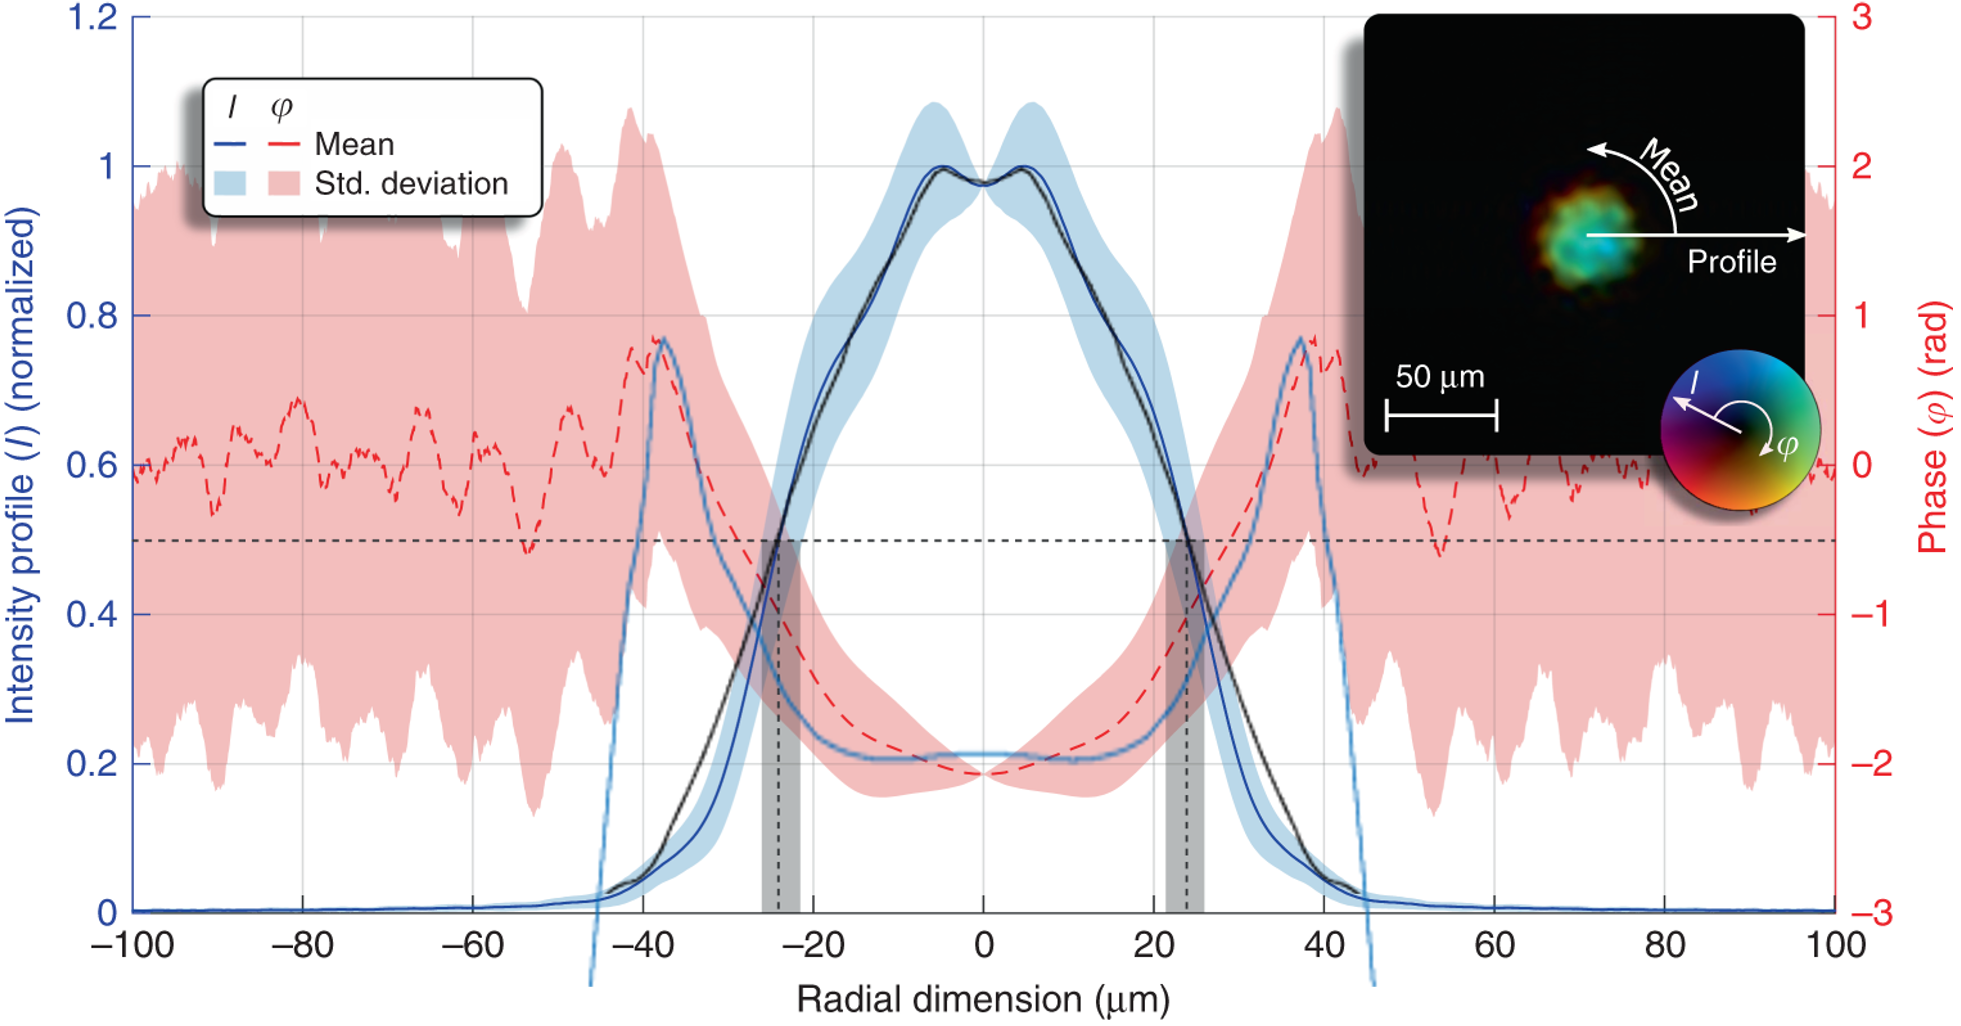
\includegraphics[width=0.75\textwidth]{Figuras/anx_cmp_81.png}
  \caption*{Comparación entre los perfiles radiales de intensidad--fase con $r_{u}=\qty{10}{µm}$, manteniendo los valores de los parámetros $r_{L}=\qty{5}{µm}$, $\sigma_{L}=\qty{15}{µm}$ y $\sigma_{u}=\qty{17}{µm}$; y el experimento.}
\end{figure}

\begin{figure}[htbp]
  \centering
  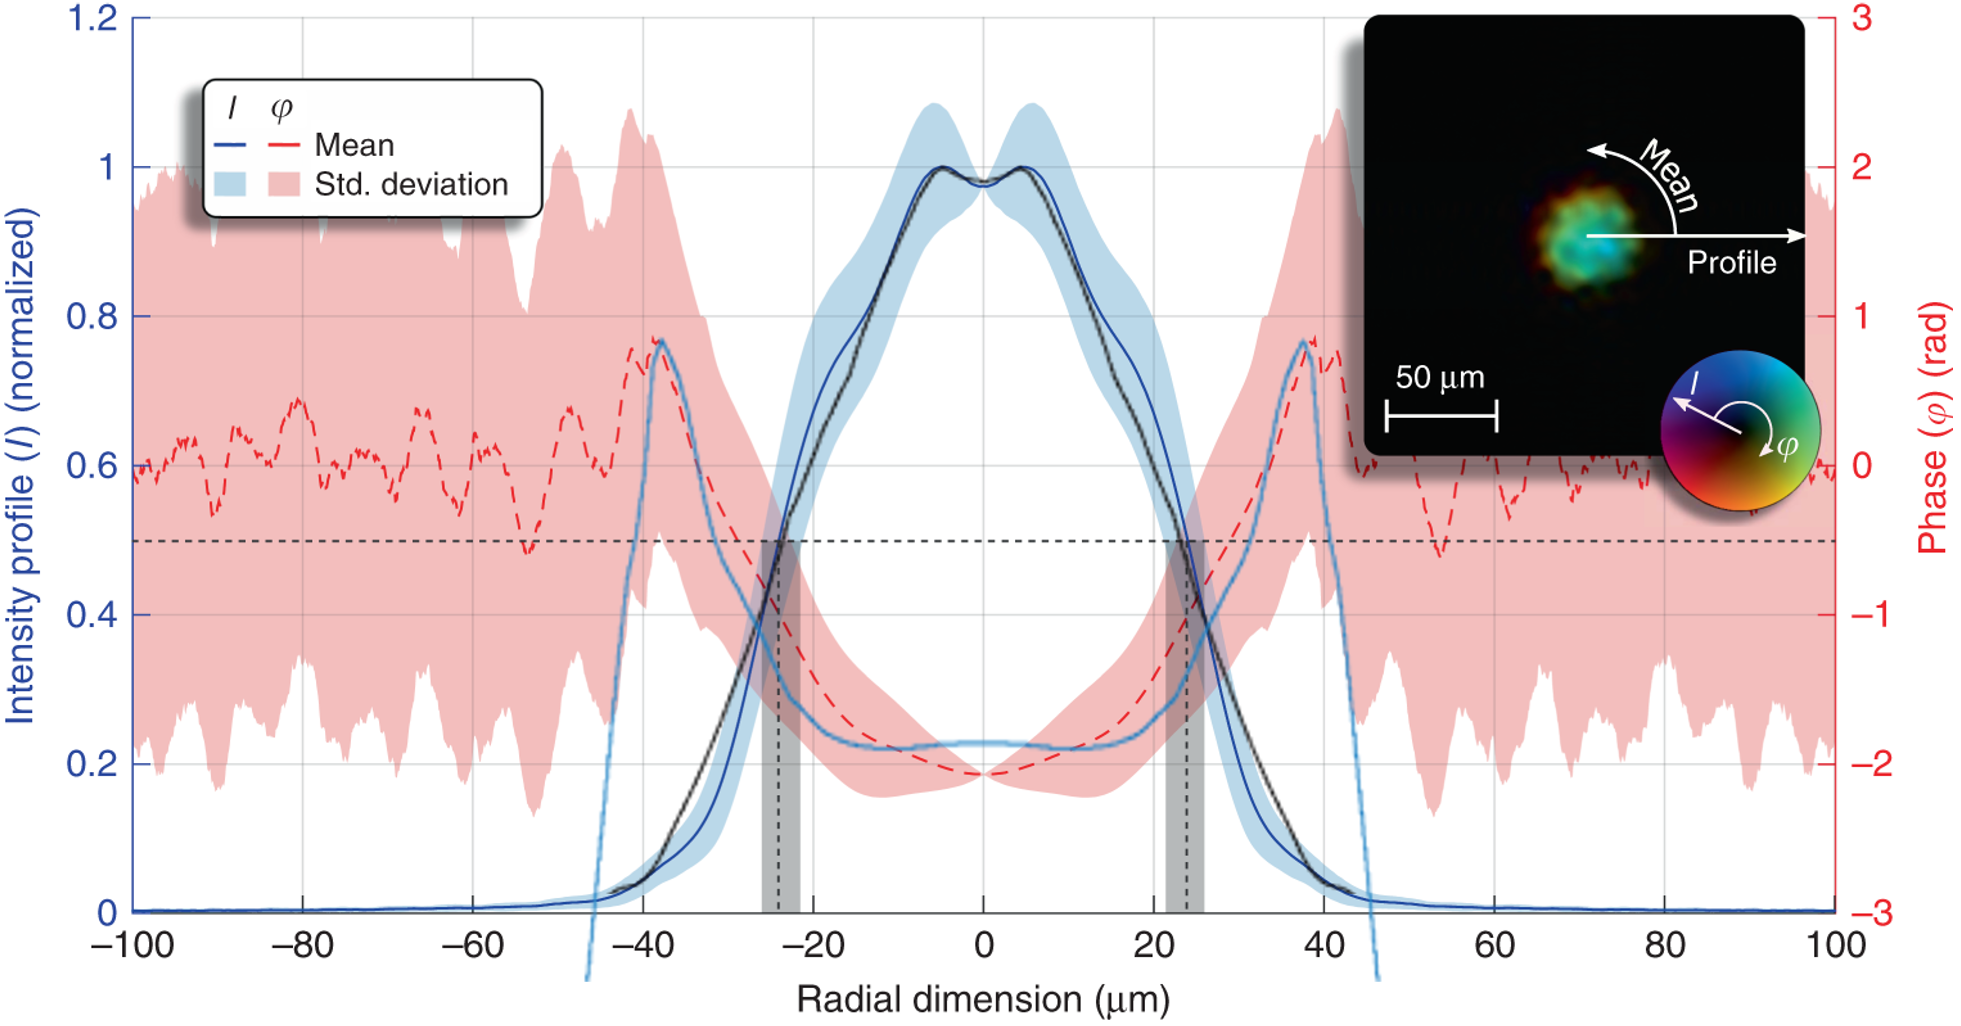
\includegraphics[width=0.75\textwidth]{Figuras/anx_cmp_82.png}
  \caption*{Comparación entre los perfiles radiales de intensidad--fase con $r_{u}=\qty{15}{µm}$, manteniendo los valores de los parámetros $r_{L}=\qty{5}{µm}$, $\sigma_{L}=\qty{15}{µm}$ y $\sigma_{u}=\qty{17}{µm}$; y el experimento.}
\end{figure}

\newpage

\begin{figure}[htbp]
  \centering
  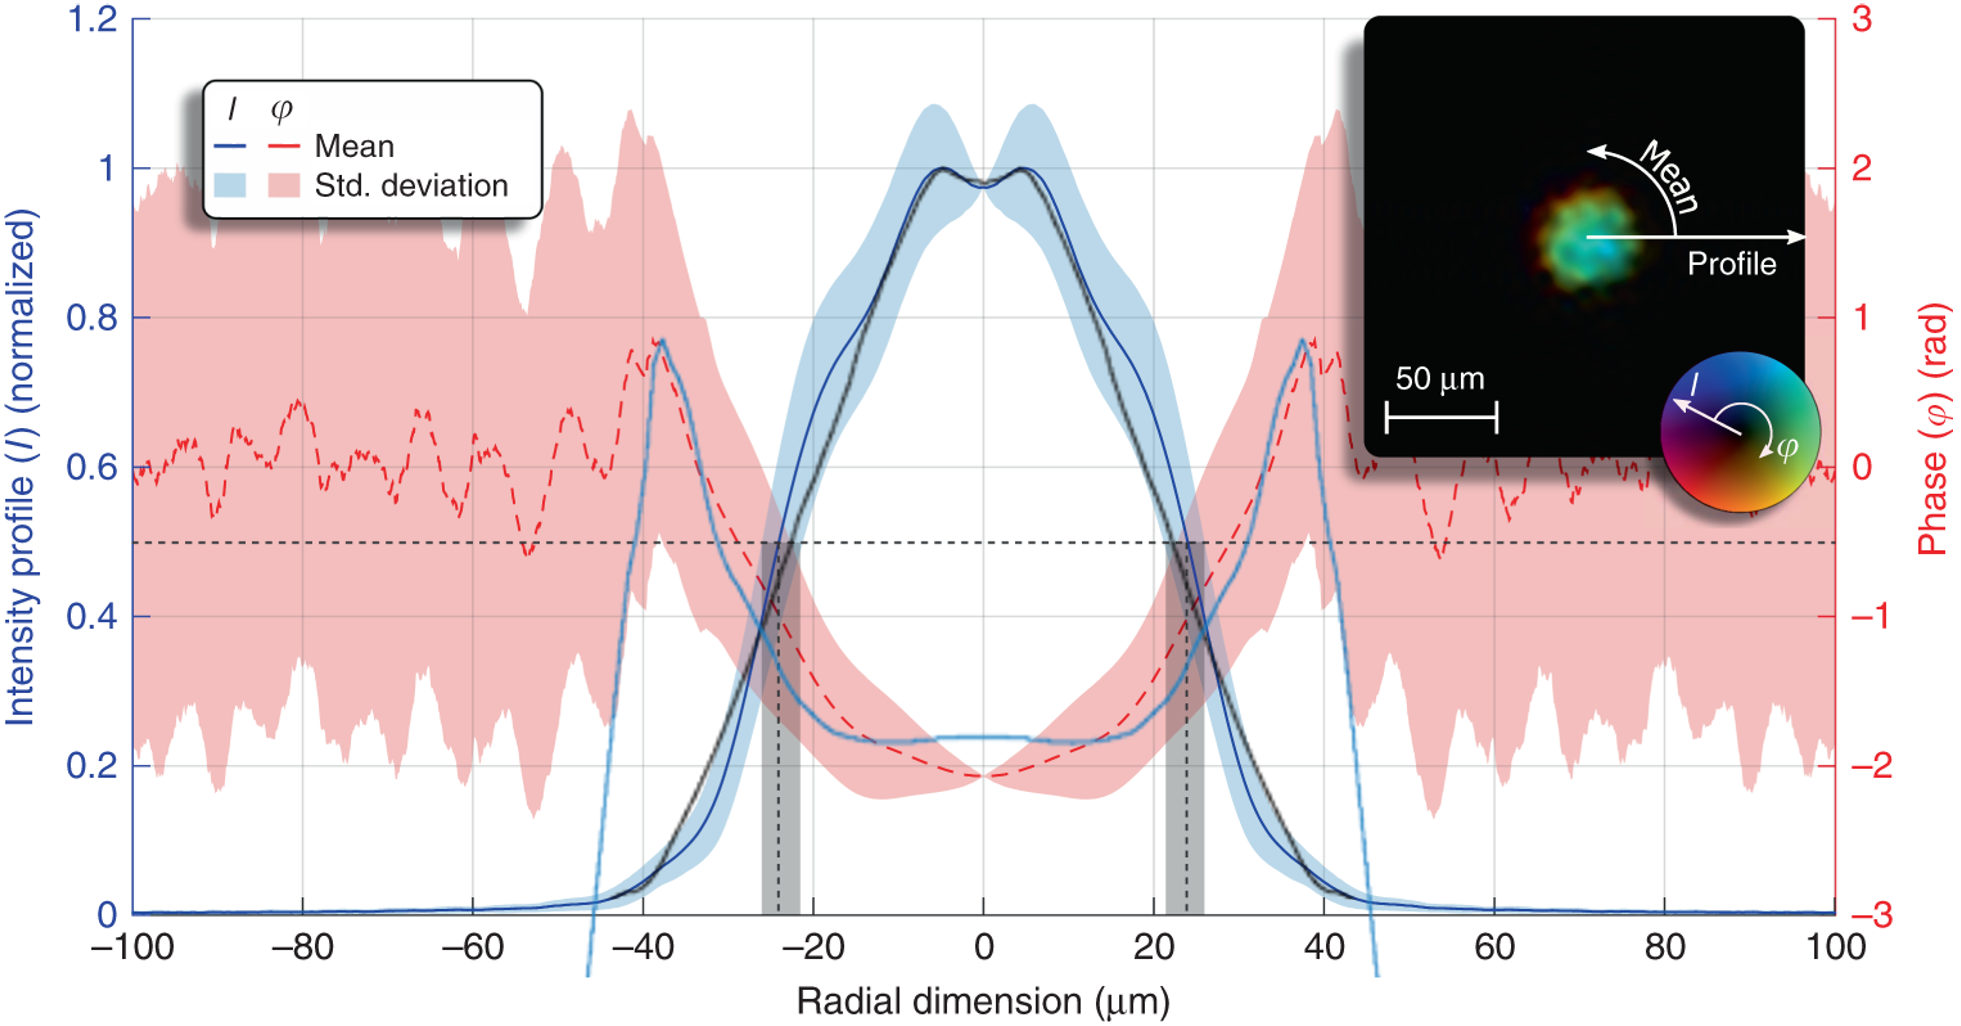
\includegraphics[width=0.7\textwidth]{Figuras/anx_cmp_83.png}
  \caption*{Comparación entre los perfiles radiales de intensidad--fase con $r_{u}=\qty{18}{µm}$, manteniendo los valores de los parámetros $r_{L}=\qty{5}{µm}$, $\sigma_{L}=\qty{15}{µm}$ y $\sigma_{u}=\qty{17}{µm}$; y el experimento.}
\end{figure}

\begin{figure}[htbp]
  \centering
  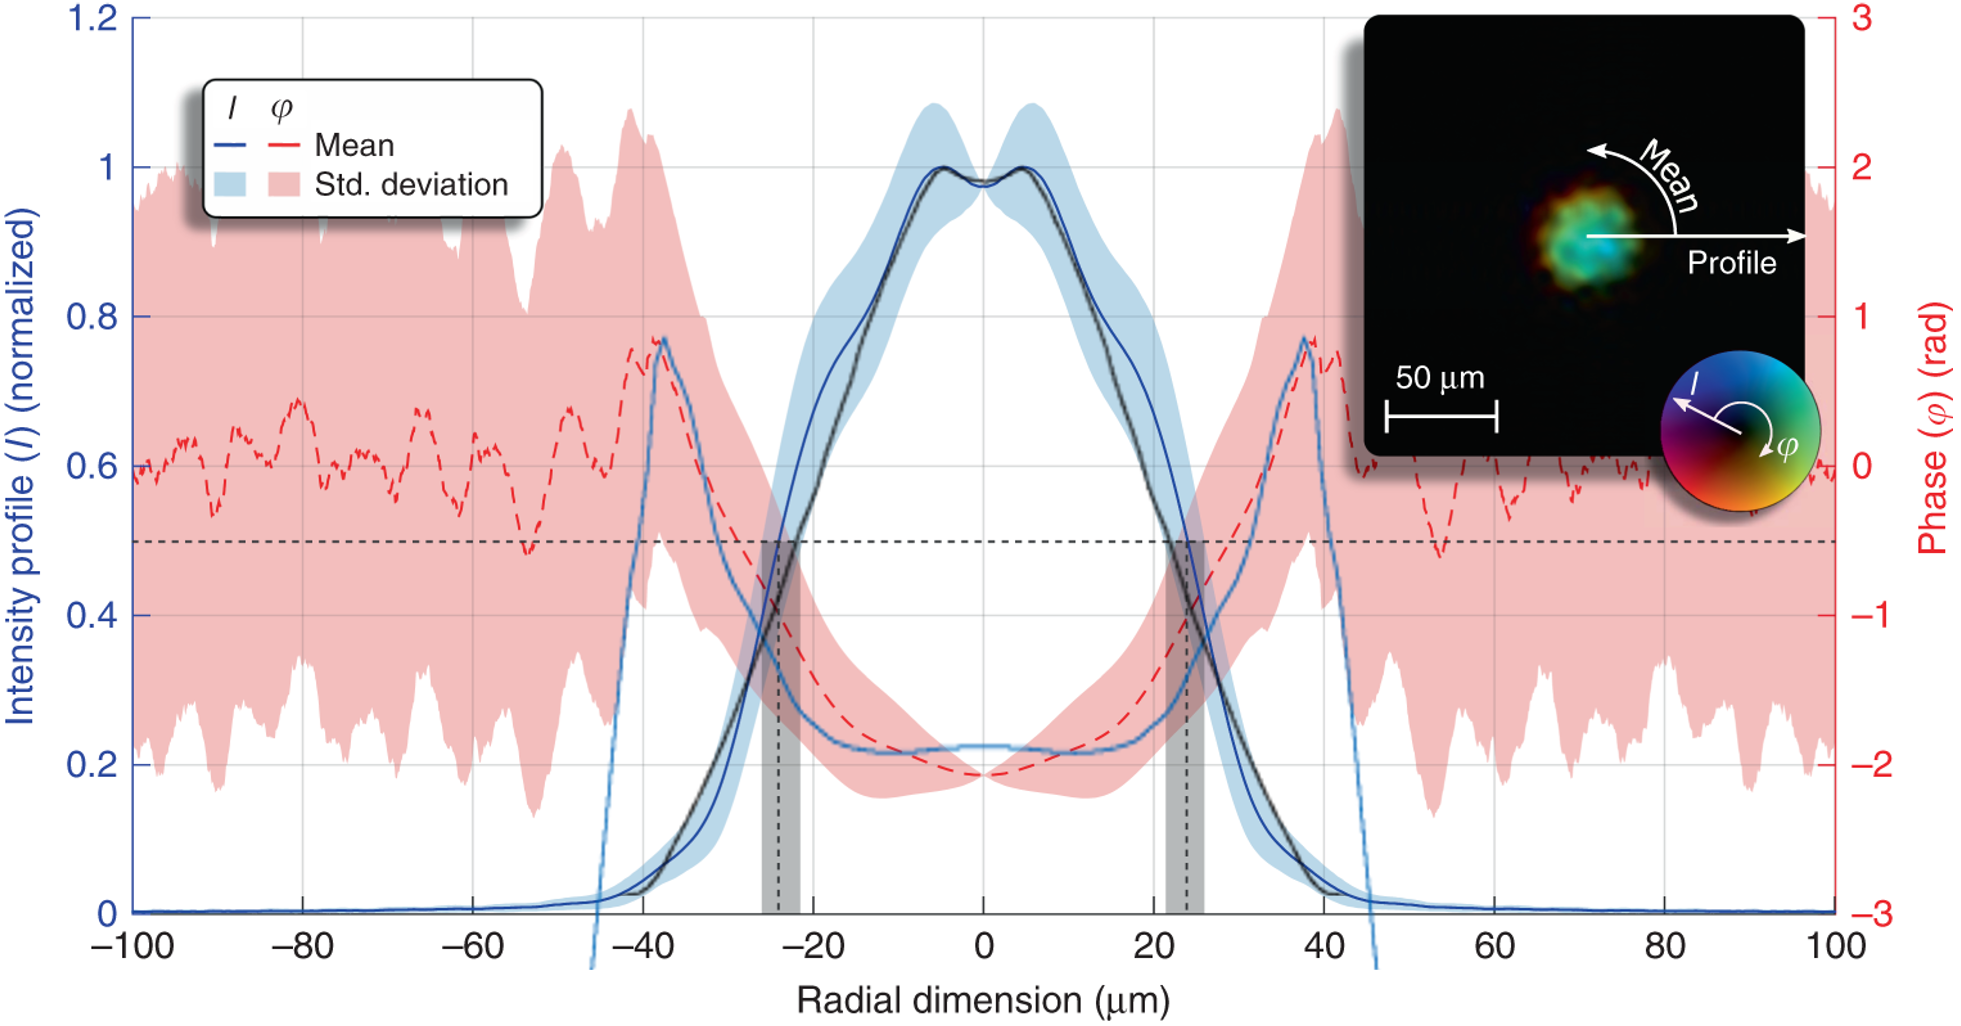
\includegraphics[width=0.74\textwidth]{Figuras/anx_cmp_84.png}
  \caption*{Comparación entre los perfiles radiales de intensidad--fase con $r_{u}=\qty{20}{µm}$, manteniendo los valores de los parámetros $r_{L}=\qty{5}{µm}$, $\sigma_{L}=\qty{15}{µm}$ y $\sigma_{u}=\qty{17}{µm}$; y el experimento.}
\end{figure}

\subsection*{Variando el parámetro \texorpdfstring{$\sigma_{u}$}{sigma-u}}

\begin{figure}[htbp!]
  \centering
  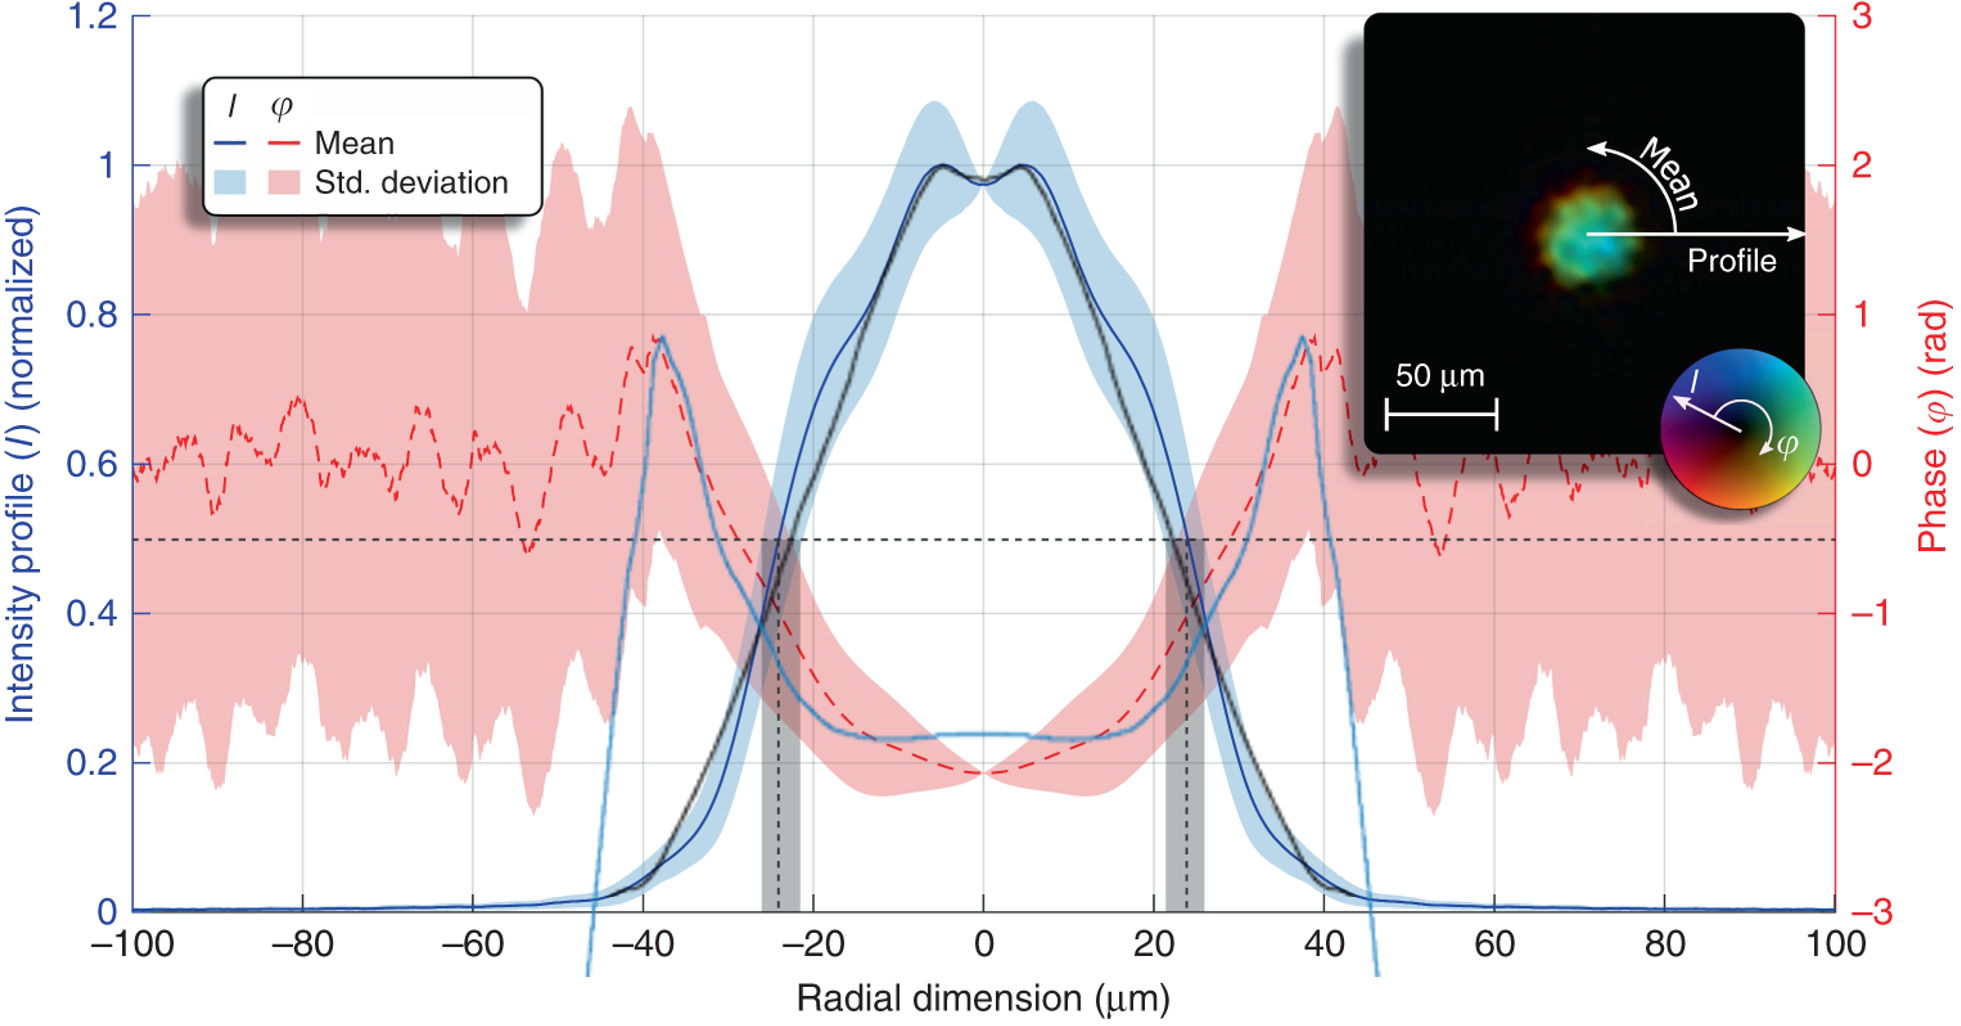
\includegraphics[width=0.74\textwidth]{Figuras/anx_cmp_91.png}
  \caption*{Comparación entre los perfiles radiales de intensidad--fase con $\sigma_{u}=\qty{17}{µm}$, manteniendo los valores de los parámetros $r_{L}=\qty{5}{µm}$, $\sigma_{L}=\qty{15}{µm}$ y $r_{u}=\qty{18}{µm}$; y el experimento.}
\end{figure}

\newpage

\begin{figure}[htbp]
  \centering
  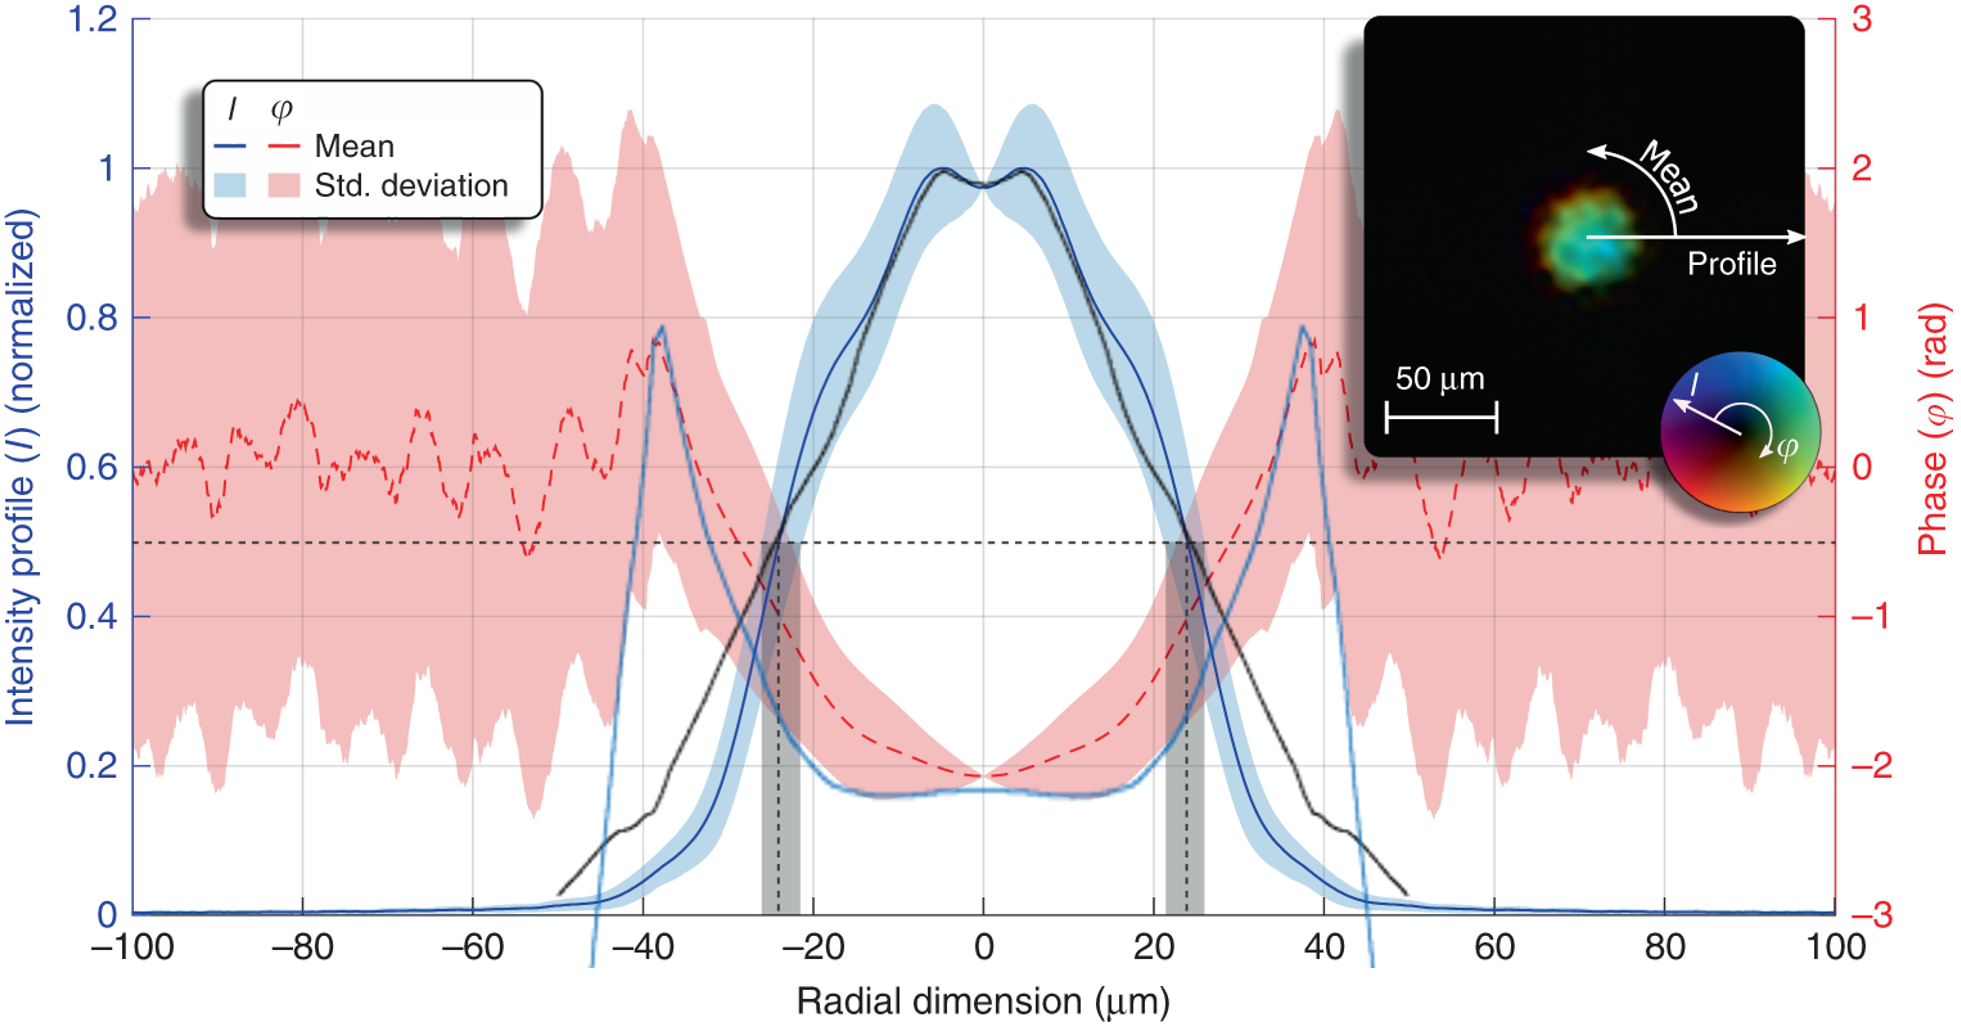
\includegraphics[width=0.75\textwidth]{Figuras/anx_cmp_92.png}
  \caption*{Comparación entre los perfiles radiales de intensidad--fase con $\sigma_{u}=\qty{20}{µm}$, manteniendo los valores de los parámetros $r_{L}=\qty{5}{µm}$, $\sigma_{L}=\qty{15}{µm}$ y $r_{u}=\qty{18}{µm}$; y el experimento.}
\end{figure}

\begin{figure}[htbp]
  \centering
  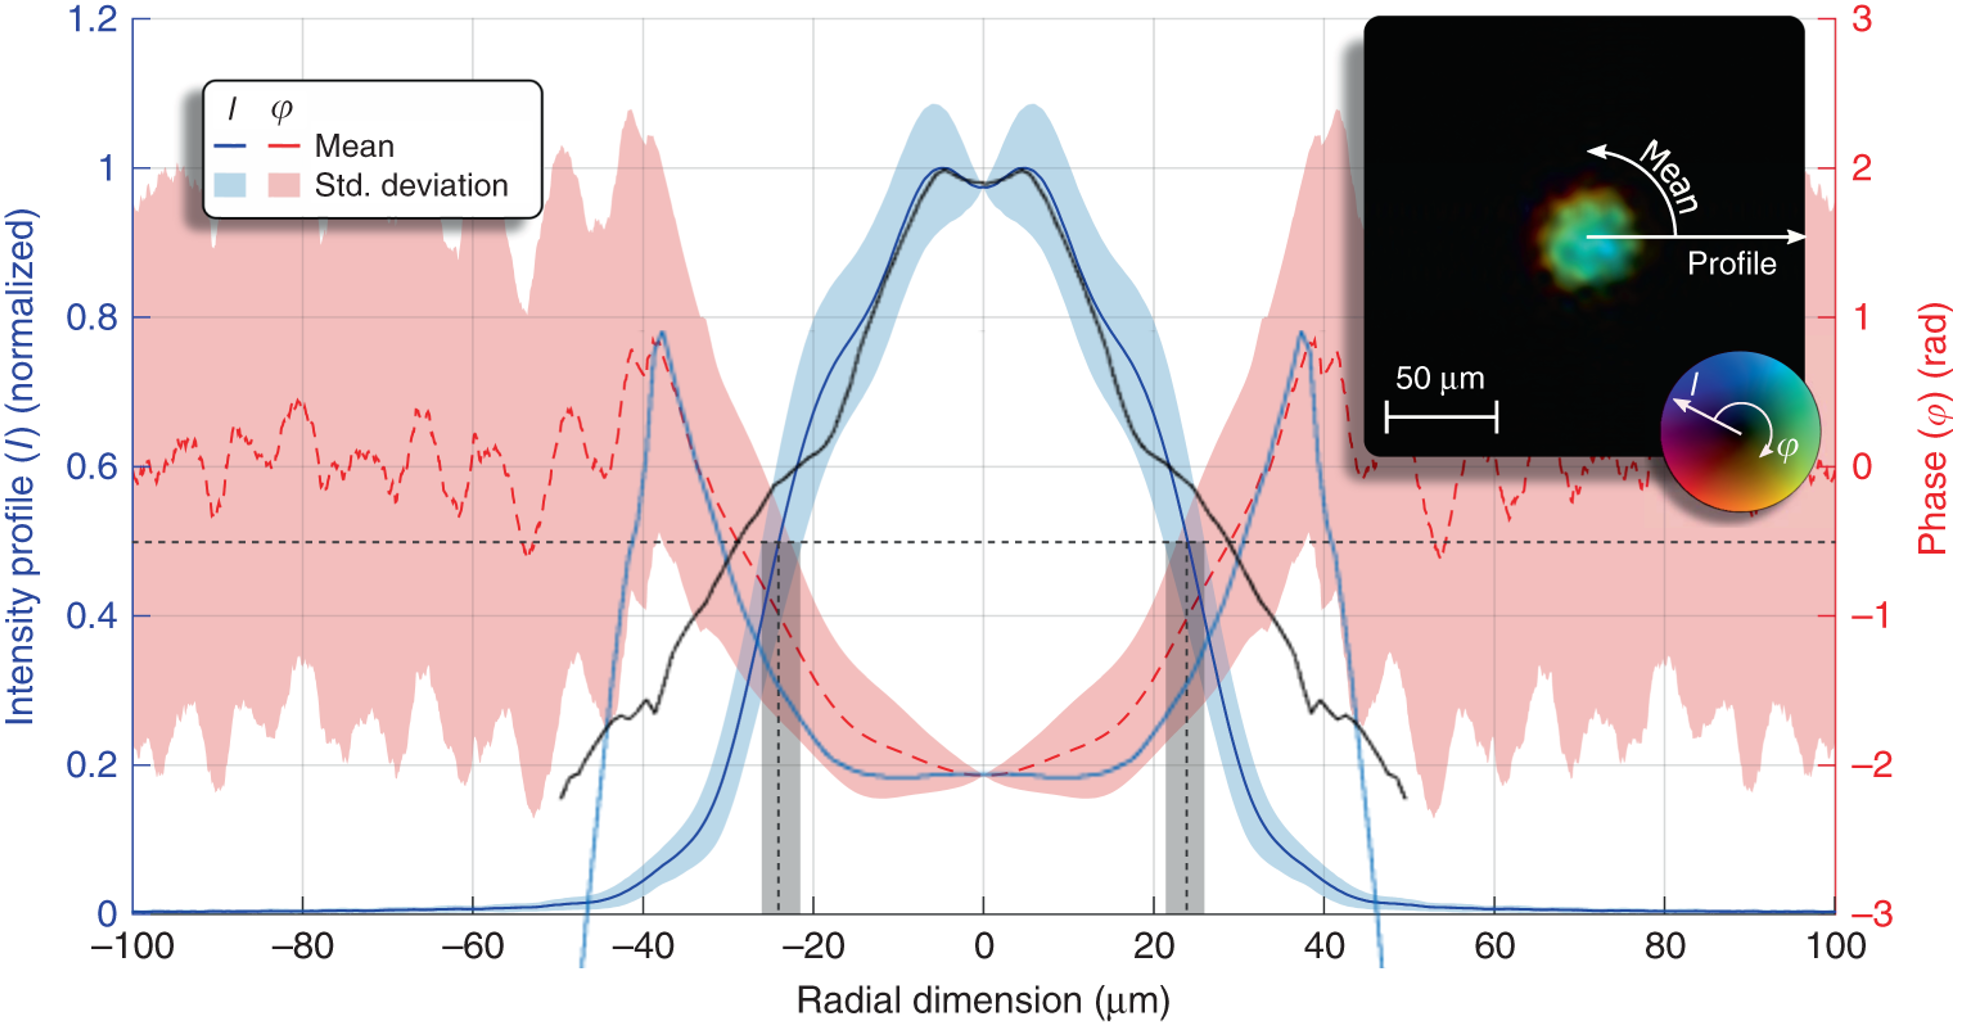
\includegraphics[width=0.75\textwidth]{Figuras/anx_cmp_93.png}
  \caption*{Comparación entre los perfiles radiales de intensidad--fase con $\sigma_{u}=\qty{25}{µm}$, manteniendo los valores de los parámetros $r_{L}=\qty{5}{µm}$, $\sigma_{L}=\qty{15}{µm}$ y $r_{u}=\qty{18}{µm}$; y el experimento.}
\end{figure}

\subsection*{Introduciendo \acrshort{oam}}

\begin{figure}[htbp!]
  \centering
  \begin{subcaptionblock}{.4\textwidth}
    \centering
    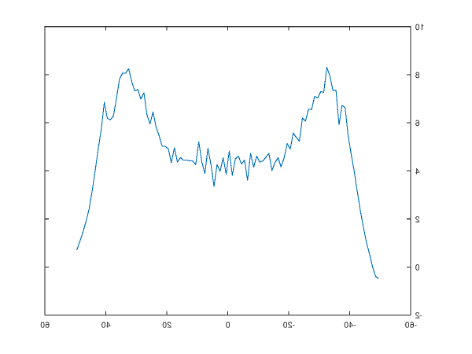
\includegraphics[width=\textwidth]{Figuras/anx_oamfs_1.png}
    \caption*{Perfil radial de intensidad (\unit{W/cm^2}) frente al radio (\unit{µm})}
  \end{subcaptionblock}
  \begin{subcaptionblock}{.4\textwidth}
    \centering
    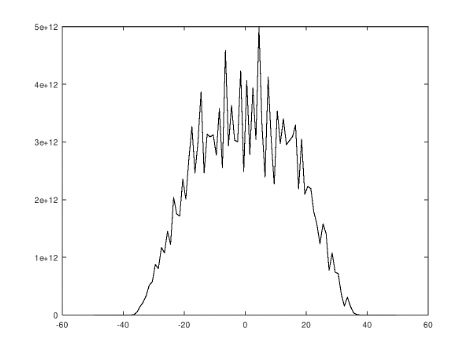
\includegraphics[width=\textwidth]{Figuras/anx_oamint_1.png}
    \caption*{Perfil radial de fase (\unit{rad}) frente al radio (\unit{µm})}
  \end{subcaptionblock}
   \caption*{Distribución radial de intensidad--fase para un haz de Laguerre--Gauss con $p=0$, $l=25$ y $\texttt{fwhm}=\qty{25}{µm}$; manteniendo $r_{L}=\qty{5}{µm}$, $r_{u}=\qty{10}{µm}$, $\sigma_{L}=\qty{15}{µm}$ y $\sigma_{u}=\qty{17}{µm}$.}
\end{figure}

\begin{figure}[htbp]
  \centering
  \begin{subcaptionblock}{.4\textwidth}
    \centering
    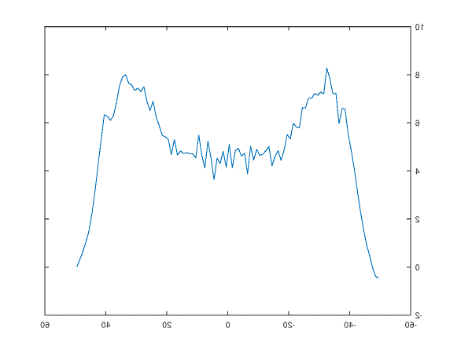
\includegraphics[width=\textwidth]{Figuras/anx_oamfs_2.png}
    \caption*{Perfil radial de intensidad (\unit{W/cm^2}) frente al radio (\unit{µm})}
  \end{subcaptionblock}
  \begin{subcaptionblock}{.4\textwidth}
    \centering
    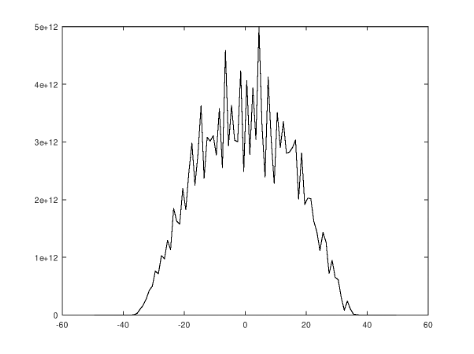
\includegraphics[width=\textwidth]{Figuras/anx_oamint_2.png}
    \caption*{Perfil radial de fase (\unit{rad}) frente al radio (\unit{µm})}
  \end{subcaptionblock}
   \caption*{Distribución radial de intensidad--fase para un haz de Laguerre--Gauss con $p=0$, $l=25$ y $\texttt{fwhm}=\qty{25}{µm}$; manteniendo $r_{L}=\qty{5}{µm}$, $r_{u}=\qty{15}{µm}$, $\sigma_{L}=\qty{15}{µm}$ y $\sigma_{u}=\qty{17}{µm}$.}
\end{figure}

\begin{figure}[htbp]
  \centering
  \begin{subcaptionblock}{.4\textwidth}
    \centering
    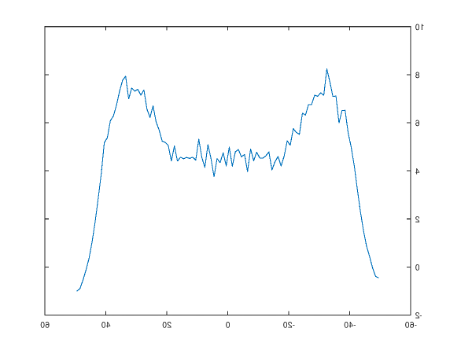
\includegraphics[width=\textwidth]{Figuras/anx_oamfs_3.png}
    \caption*{Perfil radial de intensidad (\unit{W/cm^2}) frente al radio (\unit{µm})}
  \end{subcaptionblock}
  \begin{subcaptionblock}{.4\textwidth}
    \centering
    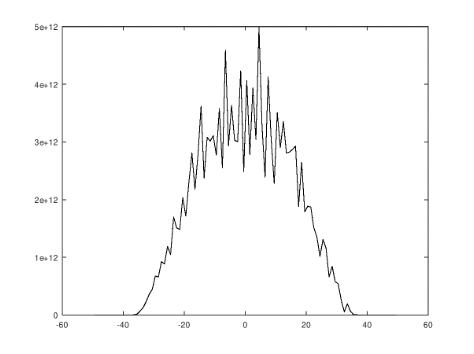
\includegraphics[width=\textwidth]{Figuras/anx_oamint_3.png}
    \caption*{Perfil radial de fase (\unit{rad}) frente al radio (\unit{µm})}
  \end{subcaptionblock}
   \caption*{Distribución radial de intensidad--fase para un haz de Laguerre--Gauss con $p=0$, $l=25$ y $\texttt{fwhm}=\qty{25}{µm}$; manteniendo $r_{L}=\qty{5}{µm}$, $r_{u}=\qty{18}{µm}$, $\sigma_{L}=\qty{15}{µm}$ y $\sigma_{u}=\qty{17}{µm}$.}
\end{figure}

\begin{figure}[htbp]
  \centering
  \begin{subcaptionblock}{.4\textwidth}
    \centering
    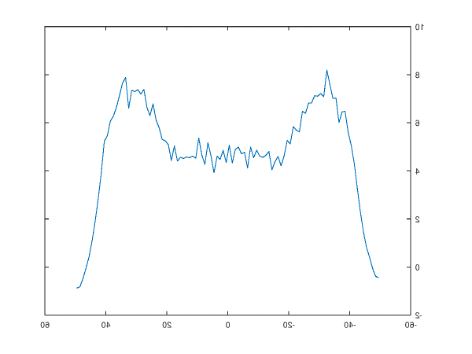
\includegraphics[width=\textwidth]{Figuras/anx_oamfs_4.png}
    \caption*{Perfil radial de intensidad (\unit{W/cm^2}) frente al radio (\unit{µm})}
  \end{subcaptionblock}
  \begin{subcaptionblock}{.4\textwidth}
    \centering
    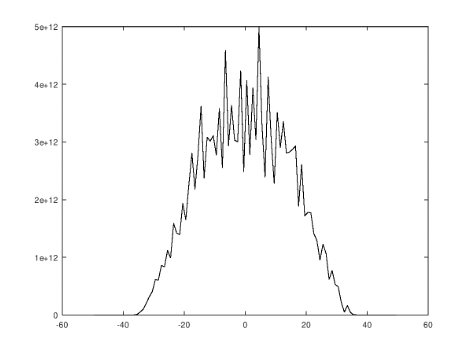
\includegraphics[width=\textwidth]{Figuras/anx_oamint_4.png}
    \caption*{Perfil radial de fase (\unit{rad}) frente al radio (\unit{µm})}
  \end{subcaptionblock}
   \caption*{Distribución radial de intensidad--fase para un haz de Laguerre--Gauss con $p=0$, $l=25$ y $\texttt{fwhm}=\qty{25}{µm}$; manteniendo $r_{L}=\qty{5}{µm}$, $r_{u}=\qty{20}{µm}$, $\sigma_{L}=\qty{15}{µm}$ y $\sigma_{u}=\qty{17}{µm}$.}
\end{figure}

\begin{figure}[htbp]
  \centering
  \begin{subcaptionblock}{.4\textwidth}
    \centering
    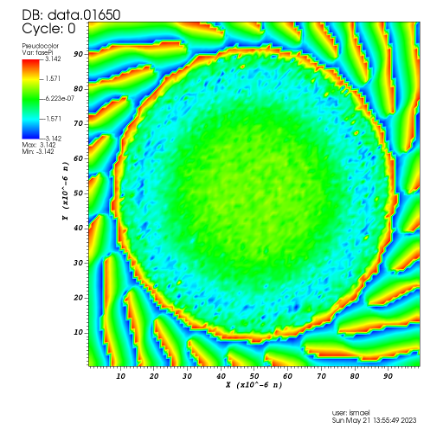
\includegraphics[width=\textwidth]{Figuras/anx_oamfs_5.png}
    \caption*{Sección transversal de fase en el plano $XY$}
  \end{subcaptionblock}
  \begin{subcaptionblock}{.4\textwidth}
    \centering
    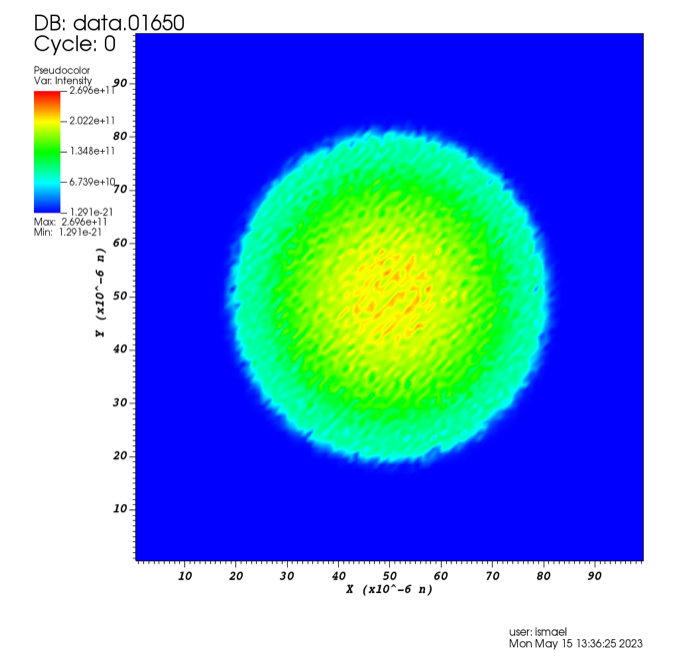
\includegraphics[width=\textwidth]{Figuras/anx_oamint_5.png}
    \caption*{Sección transversal de intensidad en el plano $XY$}
  \end{subcaptionblock}
   \caption*{Secciones transversales de intensidad--fase del pulso de Laguerre-Gauss con $p=0$, $l=25$ y $\texttt{fwhm}=\qty{25}{µm}$; manteniendo $r_{L}=\qty{5}{µm}$, $r_{u}=\qty{15}{µm}$, $\sigma_{L}=\qty{15}{µm}$ y $\sigma_{u}=\qty{17}{µm}$.}
\end{figure}

\begin{figure}[htbp]
  \centering
  \begin{subcaptionblock}{.4\textwidth}
    \centering
    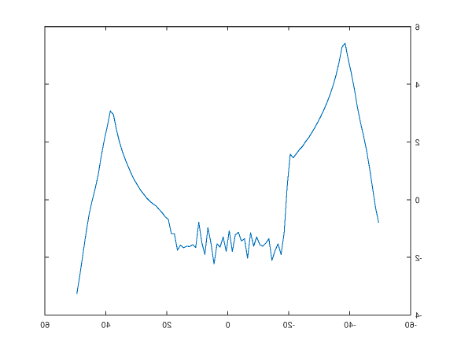
\includegraphics[width=\textwidth]{Figuras/anx_oamfs_6.png}
    \caption*{Perfil radial de intensidad (\unit{W/cm^2}) frente al radio (\unit{µm})}
  \end{subcaptionblock}
  \begin{subcaptionblock}{.4\textwidth}
    \centering
    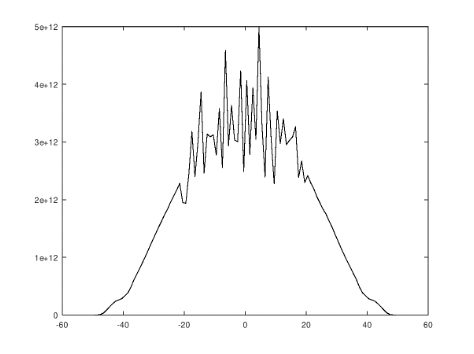
\includegraphics[width=\textwidth]{Figuras/anx_oamint_6.png}
    \caption*{Perfil radial de fase (\unit{rad}) frente al radio (\unit{µm})}
  \end{subcaptionblock}
   \caption*{Distribución radial de intensidad--fase para un haz de Laguerre--Gauss con $p=0$, $l=25$ y $\texttt{fwhm}=\qty{50}{µm}$; manteniendo $r_{L}=\qty{5}{µm}$, $r_{u}=\qty{10}{µm}$, $\sigma_{L}=\qty{15}{µm}$ y $\sigma_{u}=\qty{17}{µm}$.}
\end{figure}

\begin{figure}[htbp]
  \centering
  \begin{subcaptionblock}{.4\textwidth}
    \centering
    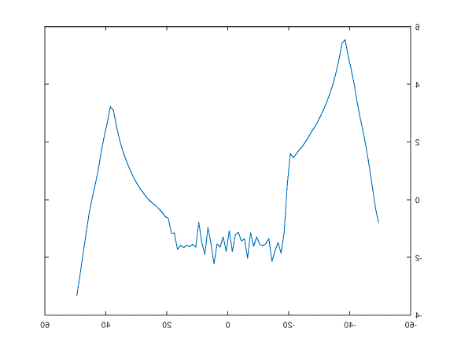
\includegraphics[width=\textwidth]{Figuras/anx_oamfs_7.png}
    \caption*{Perfil radial de intensidad (\unit{W/cm^2}) frente al radio (\unit{µm})}
  \end{subcaptionblock}
  \begin{subcaptionblock}{.4\textwidth}
    \centering
    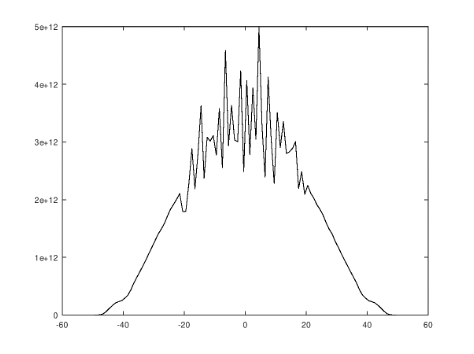
\includegraphics[width=\textwidth]{Figuras/anx_oamint_7.png}
    \caption*{Perfil radial de fase (\unit{rad}) frente al radio (\unit{µm})}
  \end{subcaptionblock}
   \caption*{Distribución radial de intensidad--fase para un haz de Laguerre--Gauss con $p=0$, $l=25$ y $\texttt{fwhm}=\qty{50}{µm}$; manteniendo $r_{L}=\qty{5}{µm}$, $r_{u}=\qty{15}{µm}$, $\sigma_{L}=\qty{15}{µm}$ y $\sigma_{u}=\qty{17}{µm}$.}
\end{figure}

\begin{figure}[htbp]
  \centering
  \begin{subcaptionblock}{.4\textwidth}
    \centering
    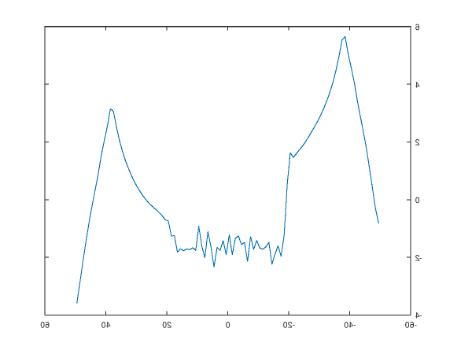
\includegraphics[width=\textwidth]{Figuras/anx_oamfs_8.png}
    \caption*{Perfil radial de intensidad (\unit{W/cm^2}) frente al radio (\unit{µm})}
  \end{subcaptionblock}
  \begin{subcaptionblock}{.4\textwidth}
    \centering
    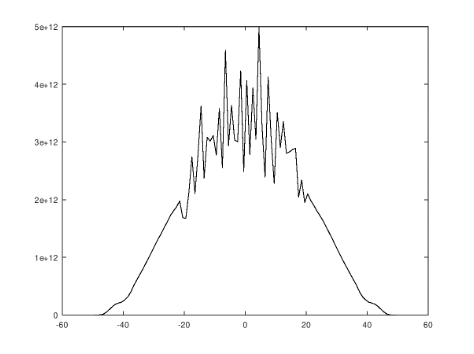
\includegraphics[width=\textwidth]{Figuras/anx_oamint_8.png}
    \caption*{Perfil radial de fase (\unit{rad}) frente al radio (\unit{µm})}
  \end{subcaptionblock}
   \caption*{Distribución radial de intensidad--fase para un haz de Laguerre--Gauss con $p=0$, $l=25$ y $\texttt{fwhm}=\qty{50}{µm}$; manteniendo $r_{L}=\qty{5}{µm}$, $r_{u}=\qty{18}{µm}$, $\sigma_{L}=\qty{15}{µm}$ y $\sigma_{u}=\qty{17}{µm}$.}
\end{figure}

\begin{figure}[htbp]
  \centering
  \begin{subcaptionblock}{.4\textwidth}
    \centering
    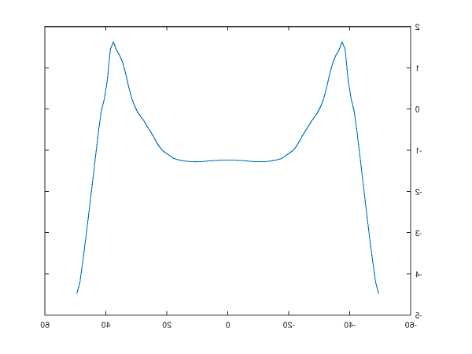
\includegraphics[width=\textwidth]{Figuras/anx_oamfs_9.png}
    \caption*{Perfil radial de intensidad (\unit{W/cm^2}) frente al radio (\unit{µm})}
  \end{subcaptionblock}
  \begin{subcaptionblock}{.4\textwidth}
    \centering
    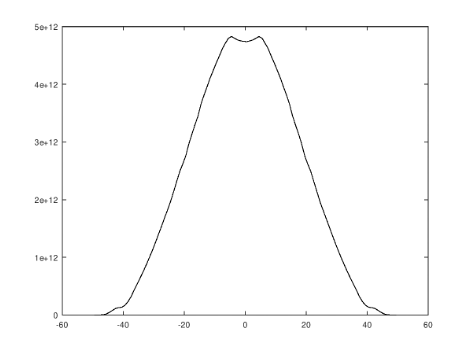
\includegraphics[width=\textwidth]{Figuras/anx_oamint_9.png}
    \caption*{Perfil radial de fase (\unit{rad}) frente al radio (\unit{µm})}
  \end{subcaptionblock}
   \caption*{Distribución radial de intensidad--fase para un haz de Laguerre--Gauss con $p=0$, $l=25$ y $\texttt{fwhm}=\qty{50}{µm}$; manteniendo $r_{L}=\qty{5}{µm}$, $r_{u}=\qty{20}{µm}$, $\sigma_{L}=\qty{15}{µm}$ y $\sigma_{u}=\qty{17}{µm}$.}
\end{figure}

\begin{figure}[htbp]
  \centering
  \begin{subcaptionblock}{.4\textwidth}
    \centering
    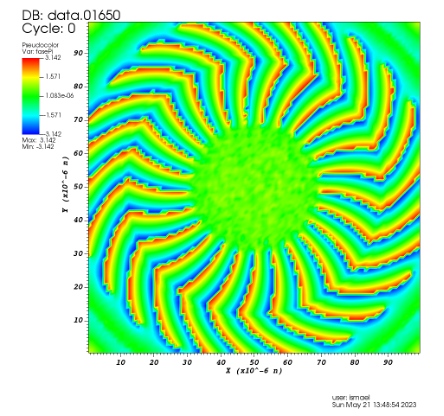
\includegraphics[width=\textwidth]{Figuras/anx_oamfs_0.png}
    \caption*{Sección transversal de fase en el plano $XY$}
  \end{subcaptionblock}
  \begin{subcaptionblock}{.4\textwidth}
    \centering
    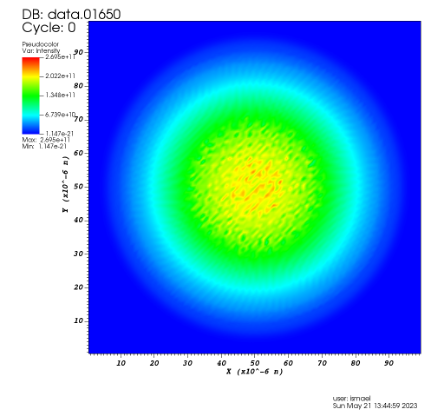
\includegraphics[width=\textwidth]{Figuras/anx_oamint_0.png}
    \caption*{Sección transversal de intensidad en el plano $XY$}
  \end{subcaptionblock}
   \caption*{Secciones transversales de intensidad--fase del pulso de Laguerre-Gauss con $p=0$, $l=25$ y $\texttt{fwhm}=\qty{50}{µm}$; manteniendo $r_{L}=\qty{5}{µm}$, $r_{u}=\qty{20}{µm}$, $\sigma_{L}=\qty{15}{µm}$ y $\sigma_{u}=\qty{17}{µm}$.}
\end{figure}
